\subsection{\acf{HOG}}
\label{sec:hog}

\ac{HOG} were first introduced by Dalal and Triggs in 2005 \cite{Dalal2005}. The idea behind \ac{HOG} is that the objects and shapes could be described by the distribution of gradients and edge directions.

The first step for extracting \ac{HOG} from images is the computation of gradients. It was evaluated that simple 1-D ($[-1, 0, 1]$) masks with a $\sigma = 0$ smoothing scale produces the best results. Color channels are computed separately and the one with the largest norm is used as the pixel's gradient vector. The authors also evaluated the usage of gamma/color normalization, but got only modest effects on performance. Gray scaling the images even reduces the performance.

The second step handles the binning by creating the cell histograms. In this step, each pixel within a $\eta \times \eta$ cell (typically 6-8 pixels as this produced the best results, regardless of the grid sizes) does a weighted vote for a histogram channel $\beta$ based on his gradient orientation. The weight of the vote is calculated by the magnitude of the gradient.

\begin{wrapfigure}[8]{r}{0.1\textwidth}
    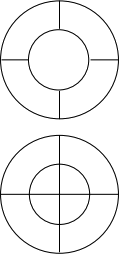
\includegraphics[width=\textwidth]{images/r-hog}
    \caption{}
    \label{fig:r-hog}
\end{wrapfigure}

As the gradient strengths vary over a wide range, based on illumination variations and foreground-background contrast, a local contrast normalization is required as a third step. This is done by grouping the histogram cells into larger blocks. The authors evaluated two grouping approaches, rectangular HOG (\acs{R-HOG}) and circular HOG (\acs{C-HOG}). \acs{R-HOG} are typical organized as $\varsigma \times \varsigma$ cell blocks (most of the time 3 or 5 blocks per direction). \acs{C-HOG} are grouped by a log-polar grid. According to the authors, at least two radial bins and four angular bins (makes a total of five to eight bins, depending if the center is also divided) as shown in figure \ref{fig:r-hog} are needed for good performance.



The authors also evaluated multiple normalization approaches to increase the detection performance.
The following approaches produced the same performance:
\begin{itemize}
	\item L2-norm $v \rightarrow v / \sqrt{||v||_2^2 + \epsilon^2}$
	\item L1-sqrt $v \rightarrow \sqrt{v / ||v||_1 + \epsilon}$
	\item L2-Hys (a L2-norm with a maximum clipping to 0.2 and a renormalization as used by Lowe \cite{Lowe2004})%$v \rightarrow \frac{\max(v / \sqrt{||v||_2^2 + \epsilon^2}, 0.2)}{\sqrt{||\max(v / \sqrt{||v||_2^2 + \epsilon^2}, 0.2)||_2^2 + \epsilon^2}}$ %TODO renormalizing 
\end{itemize}
Whilst a simple L1-norm reduced the performance by 5\% and omitting the normalization completely reduced it by 27\% according to Dalal and Triggs \cite{Dalal2005}. Another approach computes the energy of a cell and its surrounding area and uses it to normalize the cell, but also decreases the performance relative to the other approaches.

\ac{HOG} features are typically visualized by creating votes for a gradient direction based on the histogram bins of a cell. This gives a visual representation which is comprehensible from a human perspective. A sample of a \ac{HOG} representation of the lena test image can be found in figure \ref{fig:lena_hog}. Figure \ref{fig:lena_hog:8x8} shows a visualization with cells containing a $8\times8$ block of pixels and figure \ref{fig:lena_hog:32x32} a much coarser representation.

\begin{figure}[h]
    \begin{subfigure}[t]{0.3\textwidth}
        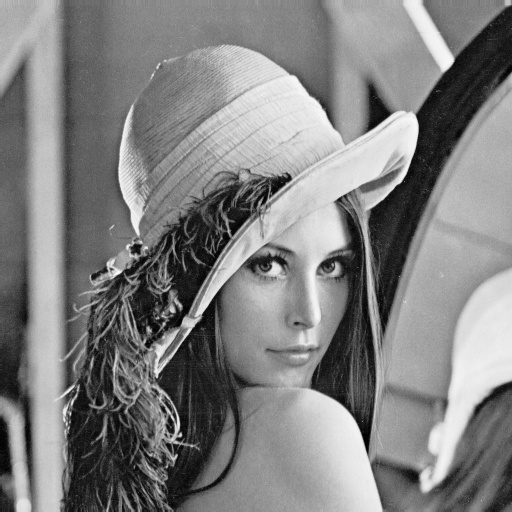
\includegraphics[width=\textwidth]{images/lena}
        \caption{Sample image in grayscale}
        \label{fig:lena_hog:lena}
    \end{subfigure}
    ~
    \begin{subfigure}[t]{0.3\textwidth}
        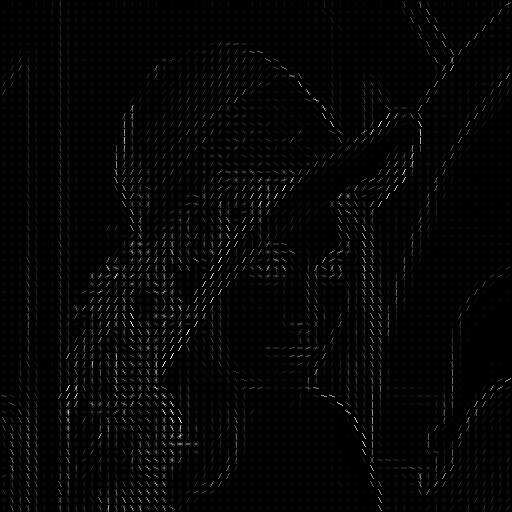
\includegraphics[width=\textwidth]{images/lena_hog_8x8}
        \caption{\acs{R-HOG} representation, $8\times8$ pixels per cell}
        \label{fig:lena_hog:8x8}
    \end{subfigure}
    ~
    \begin{subfigure}[t]{0.3\textwidth}
        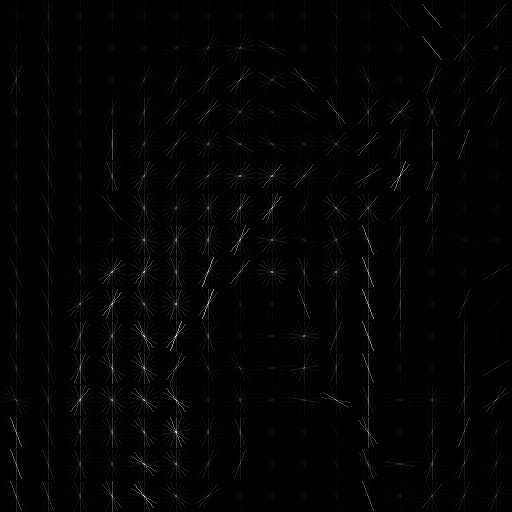
\includegraphics[width=\textwidth]{images/lena_hog_32x32}
        \caption{\acs{R-HOG} representation, $32\times32$ pixels per cell (equivalent to a downscale by 4)}
        \label{fig:lena_hog:32x32}
    \end{subfigure}
    \caption{Visualization of \ac{HOG} features}
    \label{fig:lena_hog}
\end{figure}

\ac{HOG} were initially used for pedestrian detection in static images, as Dalal and Triggs observed that the movement of individual body parts could be ignored if a general upright position is in place. Later experiments showed that it also provided good performances in other categories \cite{Malisiewicz2011}.